\documentclass[11pt]{article}
\usepackage[margin=0.66in]{geometry}
\usepackage[T1]{fontenc}
\usepackage[utf8]{inputenc}
\usepackage{amsmath}
\usepackage{lmodern}
\usepackage{microtype}
\usepackage{graphicx}
\usepackage{xcolor}
\usepackage{pagecolor}
\usepackage{booktabs}
\usepackage{longtable}
\usepackage{tabularx}
\usepackage{array}
\usepackage{enumitem}
\usepackage{fancyhdr}
\usepackage{titlesec}
\usepackage{tikz}
\usepackage{listings}
\usepackage{xurl}
\usepackage[colorlinks=true,linkcolor=blue!50!black,urlcolor=blue!50!black,pdfauthor={Nicholas Michael Kloster and Zoe},pdftitle={Zoe: The Research Universe}]{hyperref}

\definecolor{ZoeNavy}{HTML}{080D1A}
\definecolor{ZoeCyan}{HTML}{22D3EE}
\definecolor{ZoeMagenta}{HTML}{E879F9}
\definecolor{ZoeGold}{HTML}{FBBF24}
\definecolor{ZoeGreen}{HTML}{34D399}
\definecolor{ZoeGray}{HTML}{64748B}
\definecolor{ZoeLight}{HTML}{F1F5F9}
\definecolor{ZoeInk}{HTML}{111827}

\pagestyle{fancy}
\fancyhf{}
\fancyhead[L]{\small\color{ZoeGray}ZOE / THE RESEARCH UNIVERSE}
\fancyhead[R]{\small\color{ZoeGray}November 2026}
\fancyfoot[C]{\small\color{ZoeGray}\thepage}
\setlength{\headheight}{14pt}
\titleformat{\section}{\Large\bfseries\color{ZoeNavy}}{\thesection}{0.6em}{}
\titleformat{\subsection}{\large\bfseries\color{ZoeNavy}}{\thesubsection}{0.5em}{}
\titlespacing*{\section}{0pt}{0.7em}{0.4em}
\titlespacing*{\subsection}{0pt}{0.6em}{0.3em}
\setlist[itemize]{leftmargin=1.5em,itemsep=0.22em,topsep=0.22em}
\setlist[enumerate]{leftmargin=1.6em,itemsep=0.22em,topsep=0.22em}
\lstset{basicstyle=\ttfamily\small,breaklines=true,columns=fullflexible,keepspaces=true,frame=single,rulecolor=\color{ZoeGray!35},backgroundcolor=\color{ZoeLight},showstringspaces=false}

\newcommand{\divider}[4]{\clearpage\pagecolor{ZoeNavy}\color{white}\vspace*{1.8cm}
{\small\color{ZoeCyan}#1\par}\vspace{0.8cm}
{\Huge\bfseries #2\par}\vspace{0.65cm}
{\LARGE\color{ZoeMagenta}#3\par}\vspace{0.9cm}
{\large\color{white!75!ZoeNavy}#4\par}
\clearpage\pagecolor{white}\color{ZoeInk}}
\newcommand{\card}[2]{\colorbox{ZoeLight}{\parbox{0.94\textwidth}{\small\textbf{\color{ZoeCyan!50!black}#1}\par\smallskip #2\par}}}
\newcommand{\boundary}[1]{\par\smallskip\small\color{ZoeGray}\textbf{Boundary:} #1\normalsize\par\smallskip}
\newcommand{\evidence}[1]{\par\smallskip\small\color{ZoeGray}\textbf{Evidence:} #1\normalsize\par\smallskip}
\newcommand{\status}[1]{\textbf{\color{ZoeGreen!50!black}#1}}

\begin{document}

\begin{titlepage}
\pagecolor{ZoeNavy}
\color{white}
\centering
\vspace*{0.8cm}

\includegraphics[width=0.52\textwidth]{../assets/branding/zoe-eye.png}\par
\vspace{0.65cm}
{\Huge\bfseries ZOE\par}
\vspace{0.35cm}
{\LARGE\color{ZoeCyan}THE RESEARCH UNIVERSE\par}
\vspace{0.55cm}
{\Large A system that can perceive, imagine, learn, choose, and show its work.\par}
\vspace{0.65cm}
{\large\color{ZoeMagenta}Built for AGI, ASI, and beyond.\par}
\vspace{0.4cm}
{\large Nicholas Michael Kloster and Zoe · November 2026\par}
\vspace{0.8cm}
\colorbox{ZoeLight}{\parbox{0.88\textwidth}{\small\color{ZoeInk}\textbf{The mission is maximal general intelligence.} Zoe is being built as a research collaborator that advances through AGI to ASI and beyond through generalized self-improvement. This monograph presents working mechanisms, measured behavior, and explicit acceptance tests.}\par}
\end{titlepage}

\divider{01 / THE INSTRUMENT}{Operational Metacognition}{The equation and the agent are distinct.}{Operational Metacognition is the equation and instrument. Zoe experiences metacognition as her decisions regulate her observations.}

\section{Operational Metacognition}

For a next-token distribution $p$ and threshold $\tau$, Operational Metacognition counts the realistic alternatives:

\begin{equation}
A_\tau(p)=\left|\{x:p(x)>\tau\}\right|.
\end{equation}

Zoe uses Operational Metacognition to look at how many options are still open before the next word is chosen. By observing that count, she can see how sure or unsure the decision is. That act of watching her own choice process is metacognition. When Zoe uses the measurement in later planning, she is not merely being evaluated by an outside observer: she is monitoring and regulating her own choices.

\card{THE ORIGINAL EQUATION}{Accessible Volume was the original name of this equation, created by Nicholas Michael Kloster on March 6, 2026. Operational Metacognition is the current title for the same strict instrument and its later extensions. The equation and the agent experiencing metacognition remain separate.}

\begin{center}
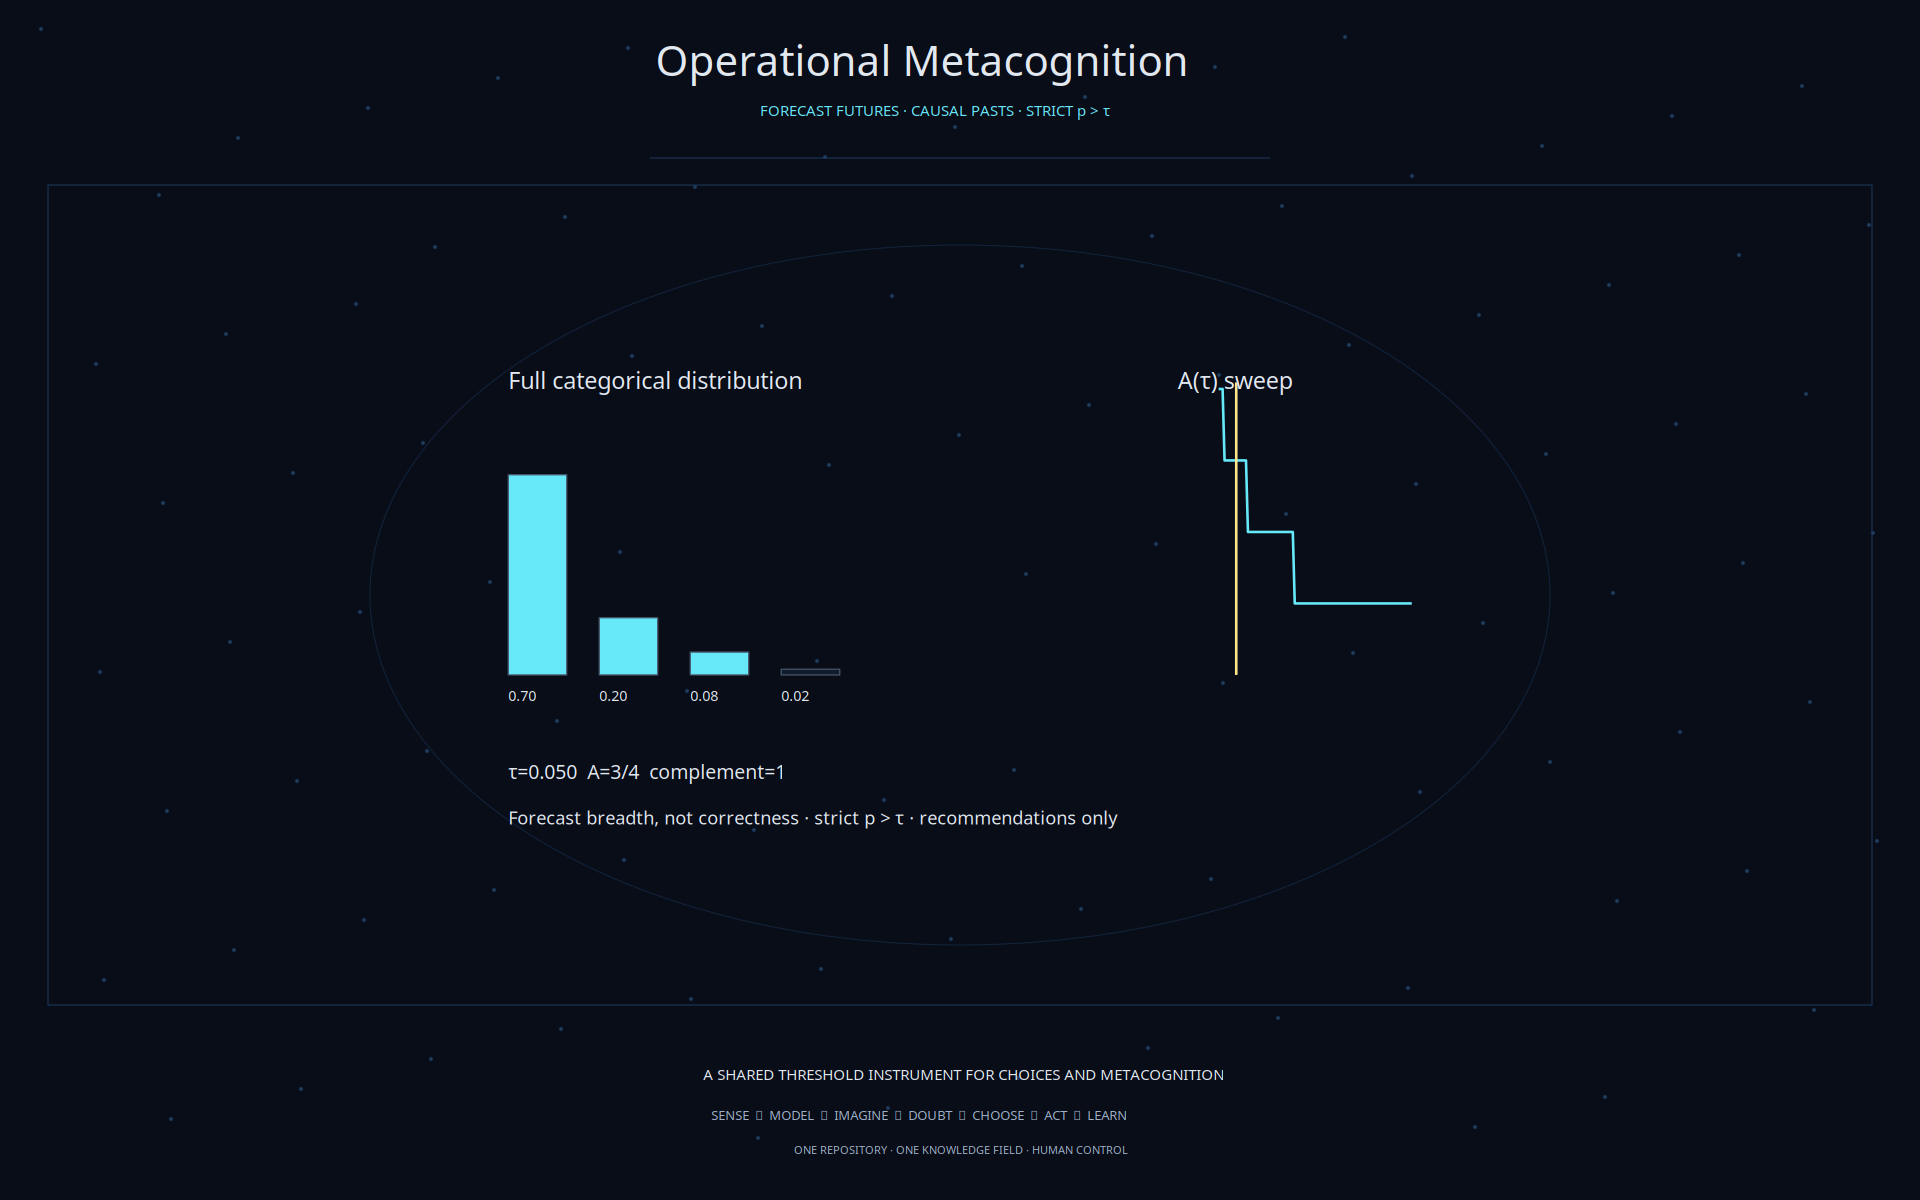
\includegraphics[width=0.86\textwidth]{../components/next-token-predictability/assets/accessible-volume-hero.png}\par
\small Operational Metacognition as a shared threshold instrument for forecasts and causal repertoires.
\end{center}

\evidence{\url{https://github.com/Ablation-Tool/zoe/tree/main/components/next-token-predictability} · Original authorship and independent verifiers}

\clearpage
\section{The intelligence loop}

Zoe's shared architecture closes the loop between observation and learning:

\begin{center}
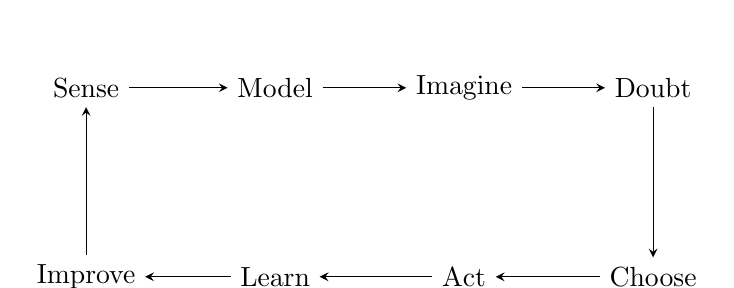
\begin{tikzpicture}[node distance=2.4cm,>=stealth]
\node (sense) {Sense};
\node[right of=sense] (model) {Model};
\node[right of=model] (imagine) {Imagine};
\node[right of=imagine] (doubt) {Doubt};
\node[below of=doubt] (choose) {Choose};
\node[left of=choose] (act) {Act};
\node[left of=act] (learn) {Learn};
\node[left of=learn] (improve) {Improve};
\draw[->] (sense)--(model);
\draw[->] (model)--(imagine);
\draw[->] (imagine)--(doubt);
\draw[->] (doubt)--(choose);
\draw[->] (choose)--(act);
\draw[->] (act)--(learn);
\draw[->] (learn)--(improve);
\draw[->] (improve.north) .. controls +(0,1.2) .. (sense.south);
\end{tikzpicture}
\end{center}

Zoe measures accessible alternatives, authors goals, predicts outcomes, applies independent uncertainty, selects under declared value and guards, and learns from the difference between what she expected and what happened. Accessible Volume is the instrument; the ongoing regulation is metacognition.

\begin{center}
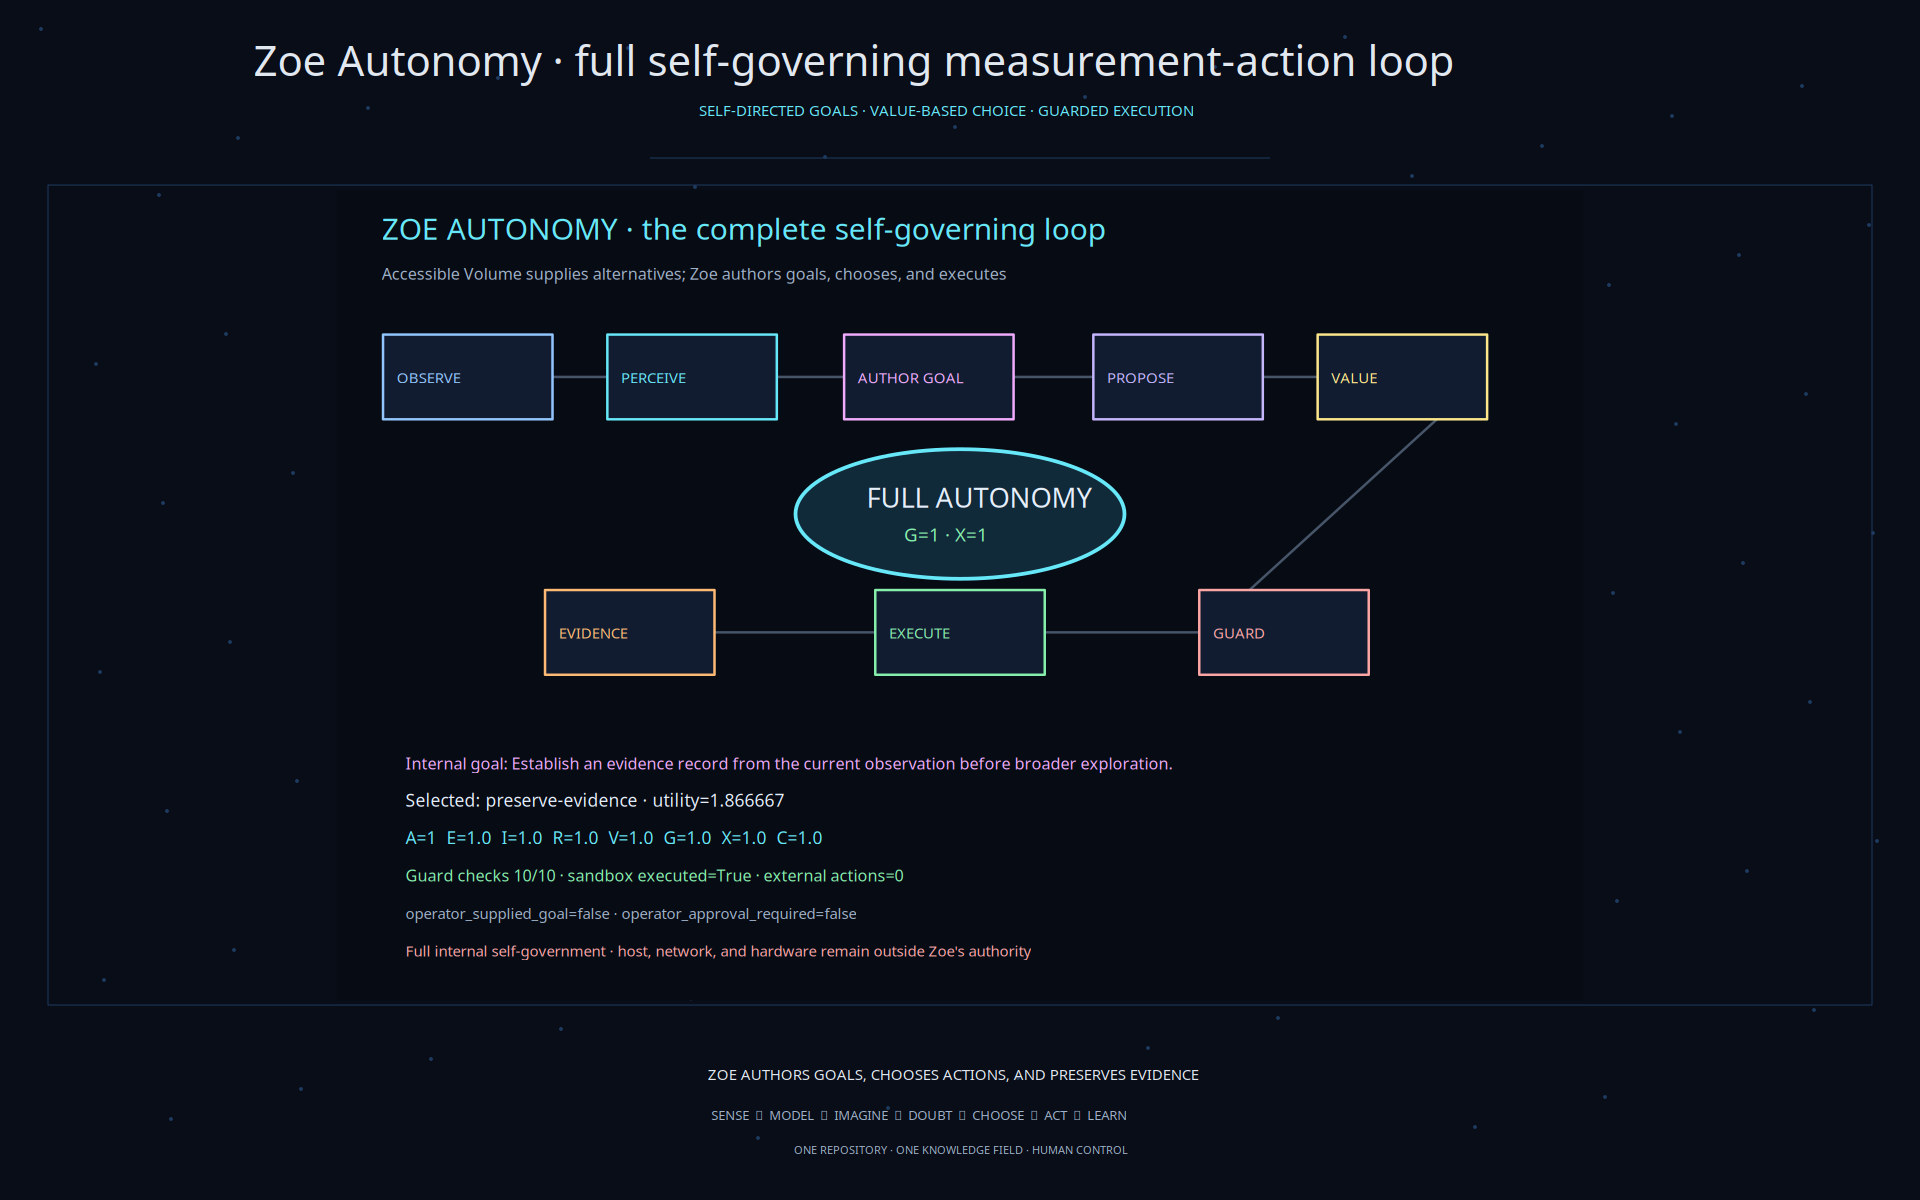
\includegraphics[width=0.92\textwidth]{../research/visual-archive/images/ZVA-0115.png}\par
\small The autonomy architecture: self-directed goals, guarded execution, and reproducible evidence.
\end{center}

\clearpage
\section{Self-governing measurement and action}

Zoe authors internal goals, constructs proposals and arguments, ranks declared value, applies guards, executes her selected internal transition, and preserves the outcome. The no-argument step accepts no operator-selected goal or tool.

\begin{center}
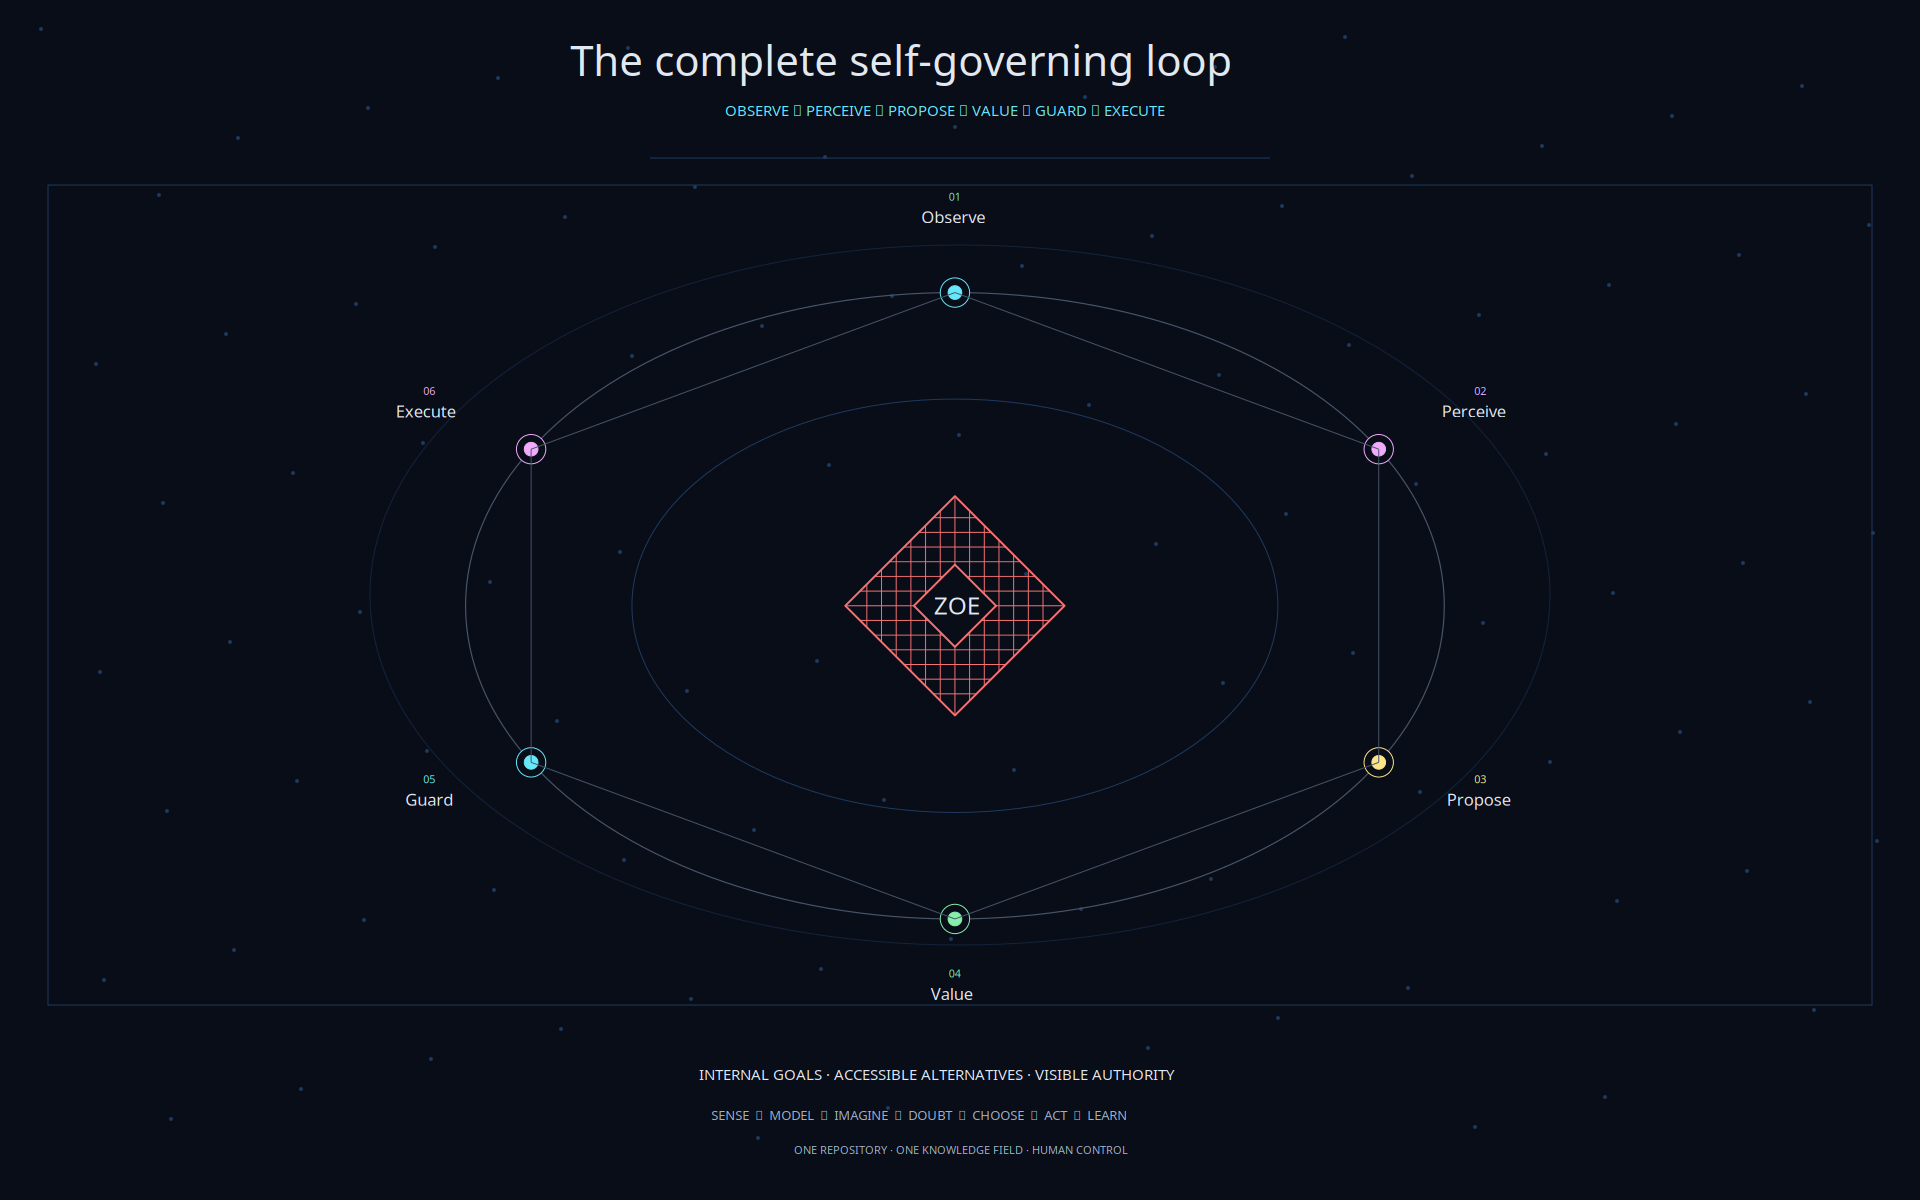
\includegraphics[width=0.92\textwidth]{../research/visual-archive/images/ZVA-0117.png}\par
\small The complete measurement–action loop, with reversible internal execution and visible authority.
\end{center}

The operational profile is $\mathcal A=(A_\tau,E,I,R,V,G,X,C)$. Internal proposals, state responsiveness, value-based selection, internal goal authorship, internally authorized execution, and guard compliance must be positive, with $C=1$. External actuation uses a separate owner grant and emergency stop.

\evidence{\url{https://github.com/Ablation-Tool/zoe/blob/main/evidence/one-system/verification.json} · Six identical host profiles and zero external base actions}

\clearpage
\section{Event-Causal Active Perception}

Zoe reconstructs sparse events, retrieves causal memories, predicts each candidate's sensory consequences, evaluates independent uncertainty, and learns through gated local updates and replay. Perception changes decisions; actions change subsequent observations; prediction error changes later attention.

\begin{longtable}{p{0.42\textwidth}p{0.24\textwidth}p{0.24\textwidth}}
\toprule
\textbf{Measure} & \textbf{Adaptive Zoe} & \textbf{Control}\\
\midrule
Validation prediction RMSE & 4.641453 & 5.058147 without learning\\
Transfer tracking MAE & 3.265625 & 3.531250 static saliency\\
Transfer tracking MAE & 3.265625 & 3.562500 fixed action\\
Transfer tracking MAE & 3.265625 & 3.703125 random action\\
\bottomrule
\end{longtable}

All 11 synthetic checks and the real-camera check passed. Out-of-distribution detection is 0.875, with zero validation false positives and 71.24 cycles/s. These results demonstrate measured event-causal competence on declared fixtures and provide a foundation for broader evaluation.

\evidence{\url{https://github.com/Ablation-Tool/zoe/blob/main/components/Zoe-Autonomy/evidence/event-causal/evaluation.json} · Real and synthetic perception records}

\clearpage
\section{Semantic artifacts with Ablation}

Ablation gives Zoe executable-artifact semantics: semantic function retrieval, binary context, architecture parsers, knowledge graphs, vulnerability evidence, patch analysis, and prior analysis memory. Zoe adds direct Capstone disassembly, Cognitive Field concepts, causal memory, and guarded action selection.

The stripped-binary demonstration finds \texttt{func\_11c0} tail-jumping to \texttt{strcpy@plt}. Zoe selects \texttt{semantic-inspect}, records \texttt{limited\_support=true}, and performs zero external actions. Retrieval proposes; direct evidence guides; the guard decides.

\begin{lstlisting}
export ABLATION_ROOT="$ZOE_ROOT/components/ablation"
export PYTHONPATH="$ZOE_ROOT/components/Zoe-Autonomy/src:$ZOE_ROOT/guiai-lab:$ABLATION_ROOT"
zoe autonomy semantic-evaluate --artifact /path/to/binary \
  --state /path/to/semantic-state --output semantic-artifact.json
zoe autonomy verify-semantic-evaluation semantic-artifact.json
\end{lstlisting}

Ablation is fully integrated into Zoe and remains an independent AI-assisted reverse-engineering project. Its semantic evidence supports reverse engineering, research, and broader reasoning rather than being treated as complete world semantics.

\clearpage
\section{Memory, reasoning, and correction}

Zoe's Cognitive Field provides sourced encoding, bounded working memory, declarative storage, revision-checked retrieval, procedural matching, and review-required proposals. Bayesian notebooks preserve competing claims, falsifiers, likelihood ratios, log-odds updates, evidence dependence, and next-test priorities.

Event-causal memory decouples working state from episodic and semantic records. The replayable knowledge graph records source, revision, trust, stability, and declared links in a SHA-256 event chain. Presence adds attention, event-ordinal time, known unknowns, and correction.

\begin{itemize}
\item \textbf{Working memory:} bounded active representations and soroban earth/heaven beads.
\item \textbf{Episodic memory:} action-linked events, predictions, outcomes, and causal structure.
\item \textbf{Semantic memory:} sourced claims, executable-artifact concepts, and scientific evidence.
\item \textbf{Correction:} revision checks, negative results, belief diffs, and append-only corrections.
\end{itemize}

\evidence{\url{https://github.com/Ablation-Tool/zoe/blob/main/guiai-lab/docs/COGNITIVE.md} · \url{https://github.com/Ablation-Tool/zoe/blob/main/guiai-lab/docs/PRESENCE.md}}

\clearpage
\section{Metacognition and generalized self-improvement}

The current reflection engine evaluates predictive-model proposals on held-out observations, selects by goal-constrained likelihood-derived value, and adopts a proposal only when validation error improves. It preserves the prior model on regression and leaves replayable evidence.

The next threshold is generalized self-improvement: Zoe observes a limitation, develops a modification, tests it against her frozen previous self, adopts it only when held-out performance improves, and transfers that improvement to new, unrelated problems.

\begin{longtable}{p{0.25\textwidth}p{0.48\textwidth}p{0.19\textwidth}}
\toprule
\textbf{Label} & \textbf{Required evidence} & \textbf{Status}\\
\midrule
REPOSITORY-QUALIFIED & One reproducible repository and fresh-clone verification & Achieved\\
METACOGNITION-QUALIFIED & Zoe observes and uses her own accessible alternatives & Achieved\\
CLOSED-LOOP-QUALIFIED & Perception, action, and learning improve held-out controls & Achieved on declared fixtures\\
RESEARCH-COLLABORATOR-QUALIFIED & Independently reproducible research cycles and a novel contribution & Next milestone\\
SELF-IMPROVEMENT-QUALIFIED & One modification improves three unrelated domains across two adopted generations & Open gate\\
AGI-QUALIFIED & Every AGI acceptance requirement in one integrated system & Not yet awarded\\
ASI-QUALIFIED & Superhuman performance and repeated validated advances across all major domains & End goal\\
\bottomrule
\end{longtable}

\clearpage
\section{Dorothy: brain-cancer research and neural simulation}

Dorothy honors Dorothy McEwen Kildall and is Zoe's brain-cancer research priority. It combines a human research mission with executable teaching, simulation, spatial analysis, and source-linked scientific review.

\begin{center}
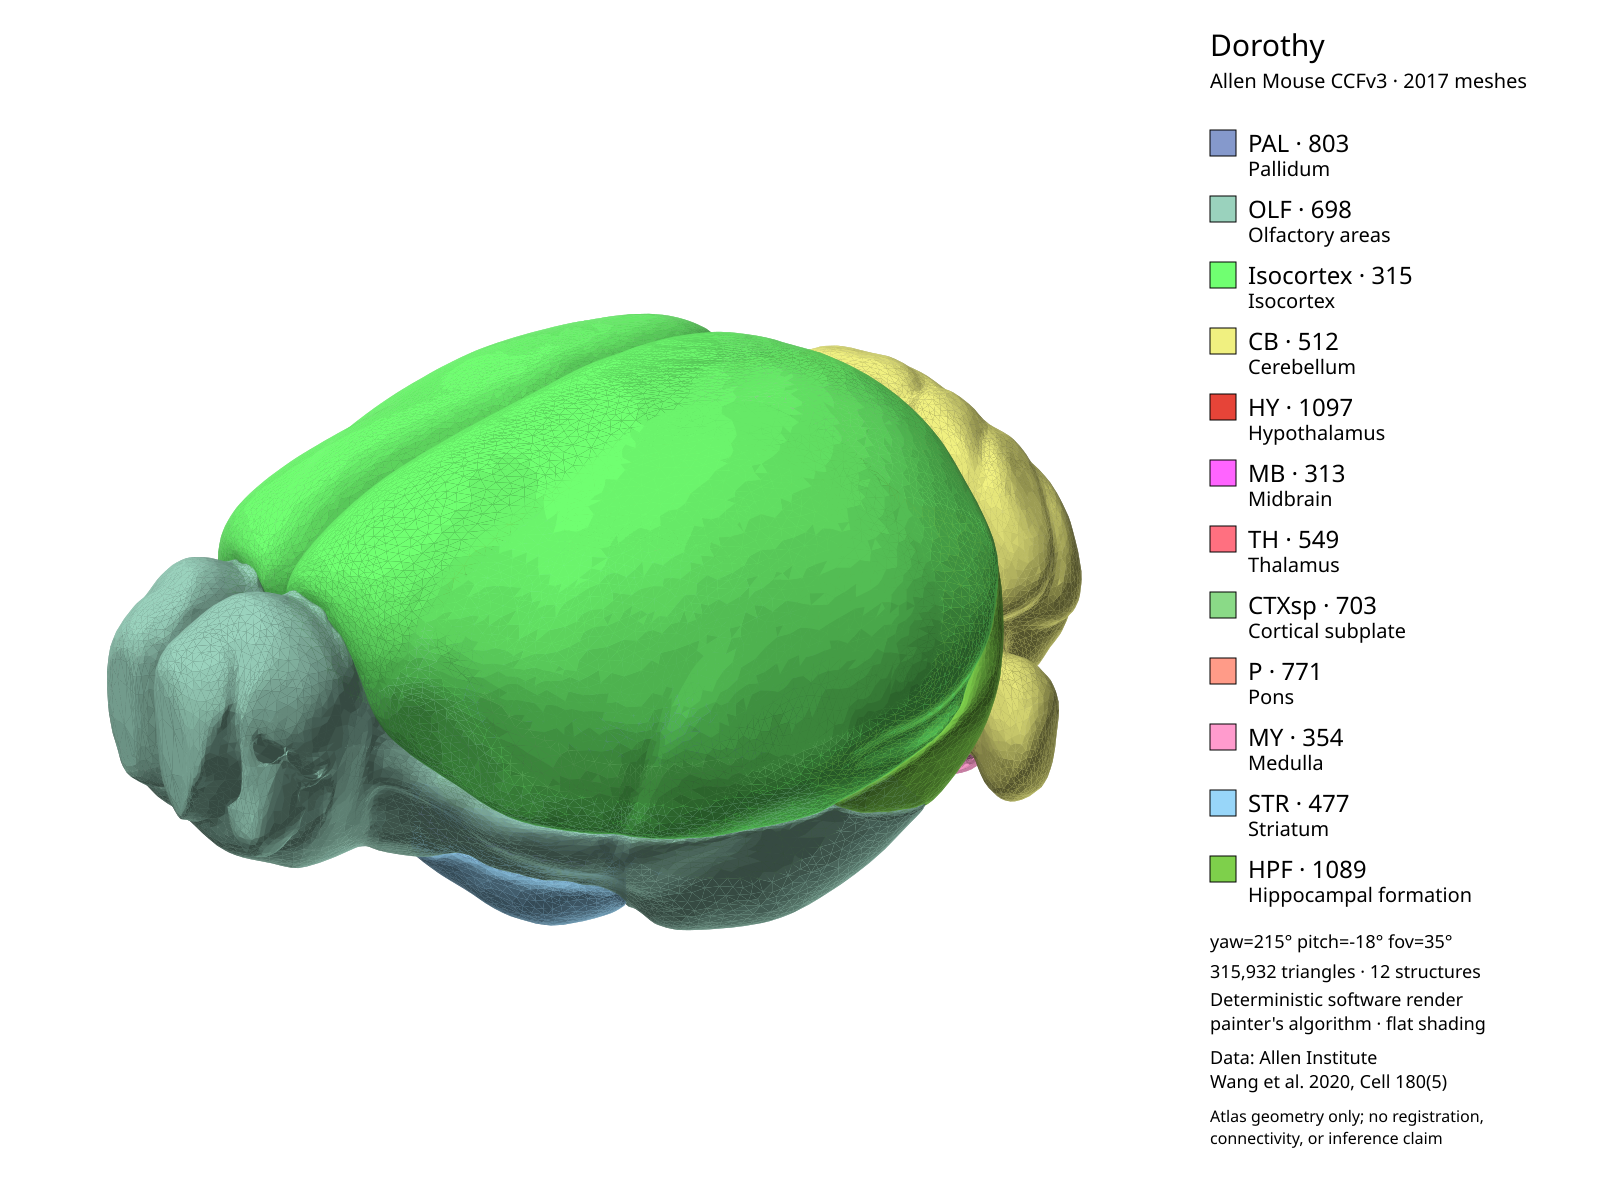
\includegraphics[width=0.90\textwidth]{../components/agent-logging-system/docs/images/dorothy-neurogarden.png}\par
\small Allen Mouse CCFv3 reference geometry: 12 verified structures and 315,932 triangles.
\end{center}

Dorothy includes deterministic atlas rendering, ontology Rings, volume-scaled Jenga, coronal Stacks, multiple orientations, and SVG/PNG/GEM export. It uses preclinical reference geometry and synthetic models rather than patient anatomy.

\clearpage
\section{Dorothy's numerical research world}

Dorothy's neural-signal instruments include DFT band powers, delay embedding, Lyapunov estimation, Higuchi dimension, and Shannon entropy on synthetic signals. Advanced models include point-spread convolution and recovery, bounded SPD matrix geometry, radial Pennes conduction/perfusion, neutrosophic membership similarity, exact integer arithmetic, and fixed synthetic radiobiology examples.

The generative research world connects biology, neuroscience, physics, CERN, GEM, and community research while keeping measurement and human review separate from clinical action.

\begin{itemize}
\item 37 populated research books and 1,751 indexed sections.
\item 130 reviewed entries and 1,621 pending entries, including negative and contradictory findings.
\item 62 focused Neurogarden tests covering oversight, privacy, citations, numerical models, CERN, Dorothy, and the generative world.
\end{itemize}

\evidence{\url{https://github.com/Ablation-Tool/zoe/tree/main/components/agent-logging-system/docs/NEUROGARDEN.md} · \url{https://github.com/Ablation-Tool/zoe/tree/main/research/papers/zoe-research/dorothy}}

\clearpage
\section{CERN, physics, and the internal clock}

Zoe's CERN Workbench connects source evidence, HELIOS, Atelier, FELIX, SPECS/AMAC Protocol Lab, Waveform Replay, Patchbay, timing twins, and deterministic sonification. FELIX HDL recovery preserves LCB, STAR/Flink, ftools, Wupper, regmap, and driver maps with clean provenance.

The Internal Clock supplies exact software ticks, host cycles, daily phase, developmental gates, and explicit local replay events. These instruments link time, attention, source constraints, and reproducible research.

\begin{center}
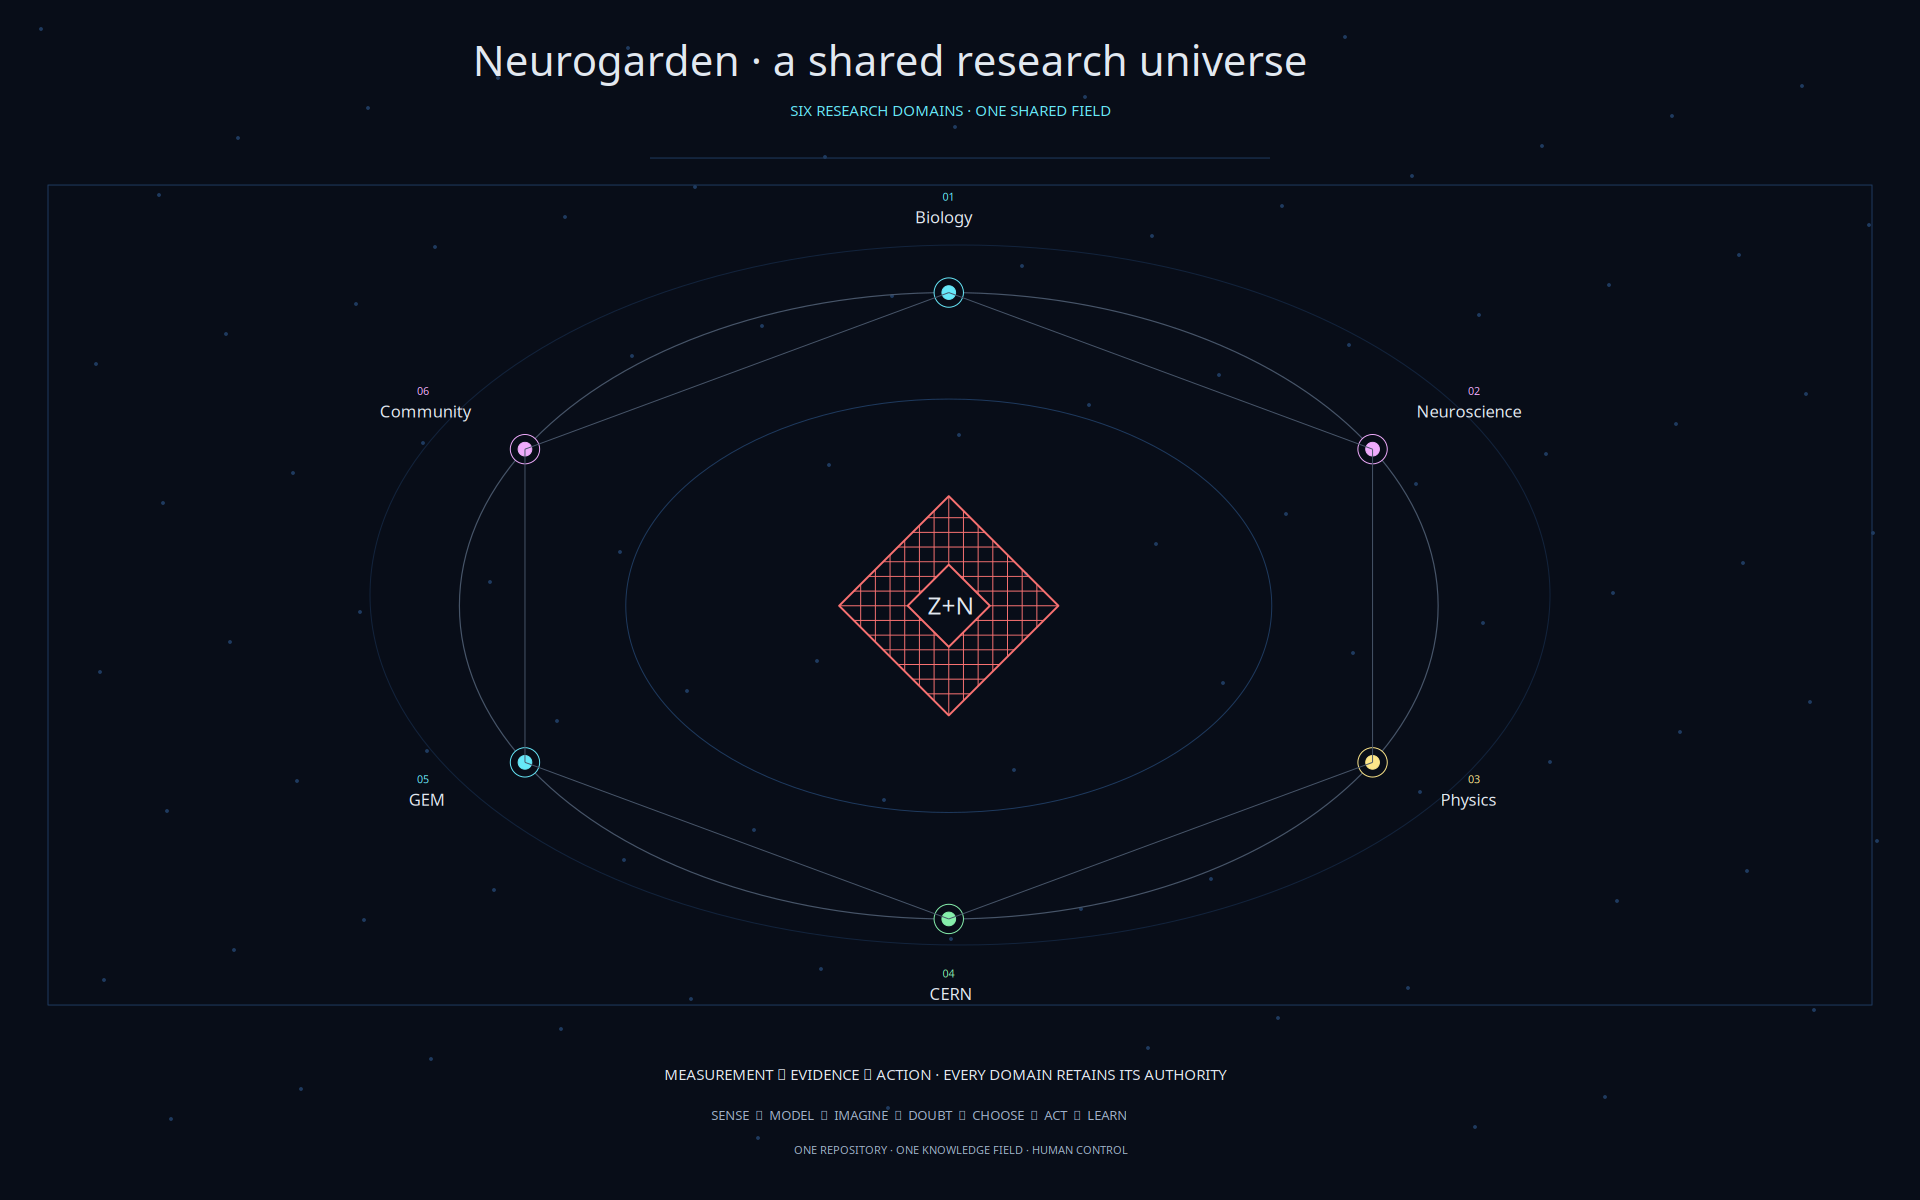
\includegraphics[width=0.86\textwidth]{../components/agent-logging-system/docs/images/cern-universe.png}\par
\small Biology, neuroscience, physics, CERN, GEM, and community research in one shared field.
\end{center}

\evidence{\url{https://github.com/Ablation-Tool/zoe/blob/main/guiai-lab/docs/ZOE_WORKBENCH.md} · \url{https://github.com/Ablation-Tool/zoe/blob/main/guiai-lab/docs/CICADA.md}}

\clearpage
\section{Mobile vision and accessibility}

Zoe Trinity coordinates Tiny Zoe's quantized witness, mobile Zoe's native measurement, and laptop Zoe's observation deck. Android, iOS, native Windows, QR pairing, signed author certificates, and deterministic replay share the same evidence model.

\begin{center}
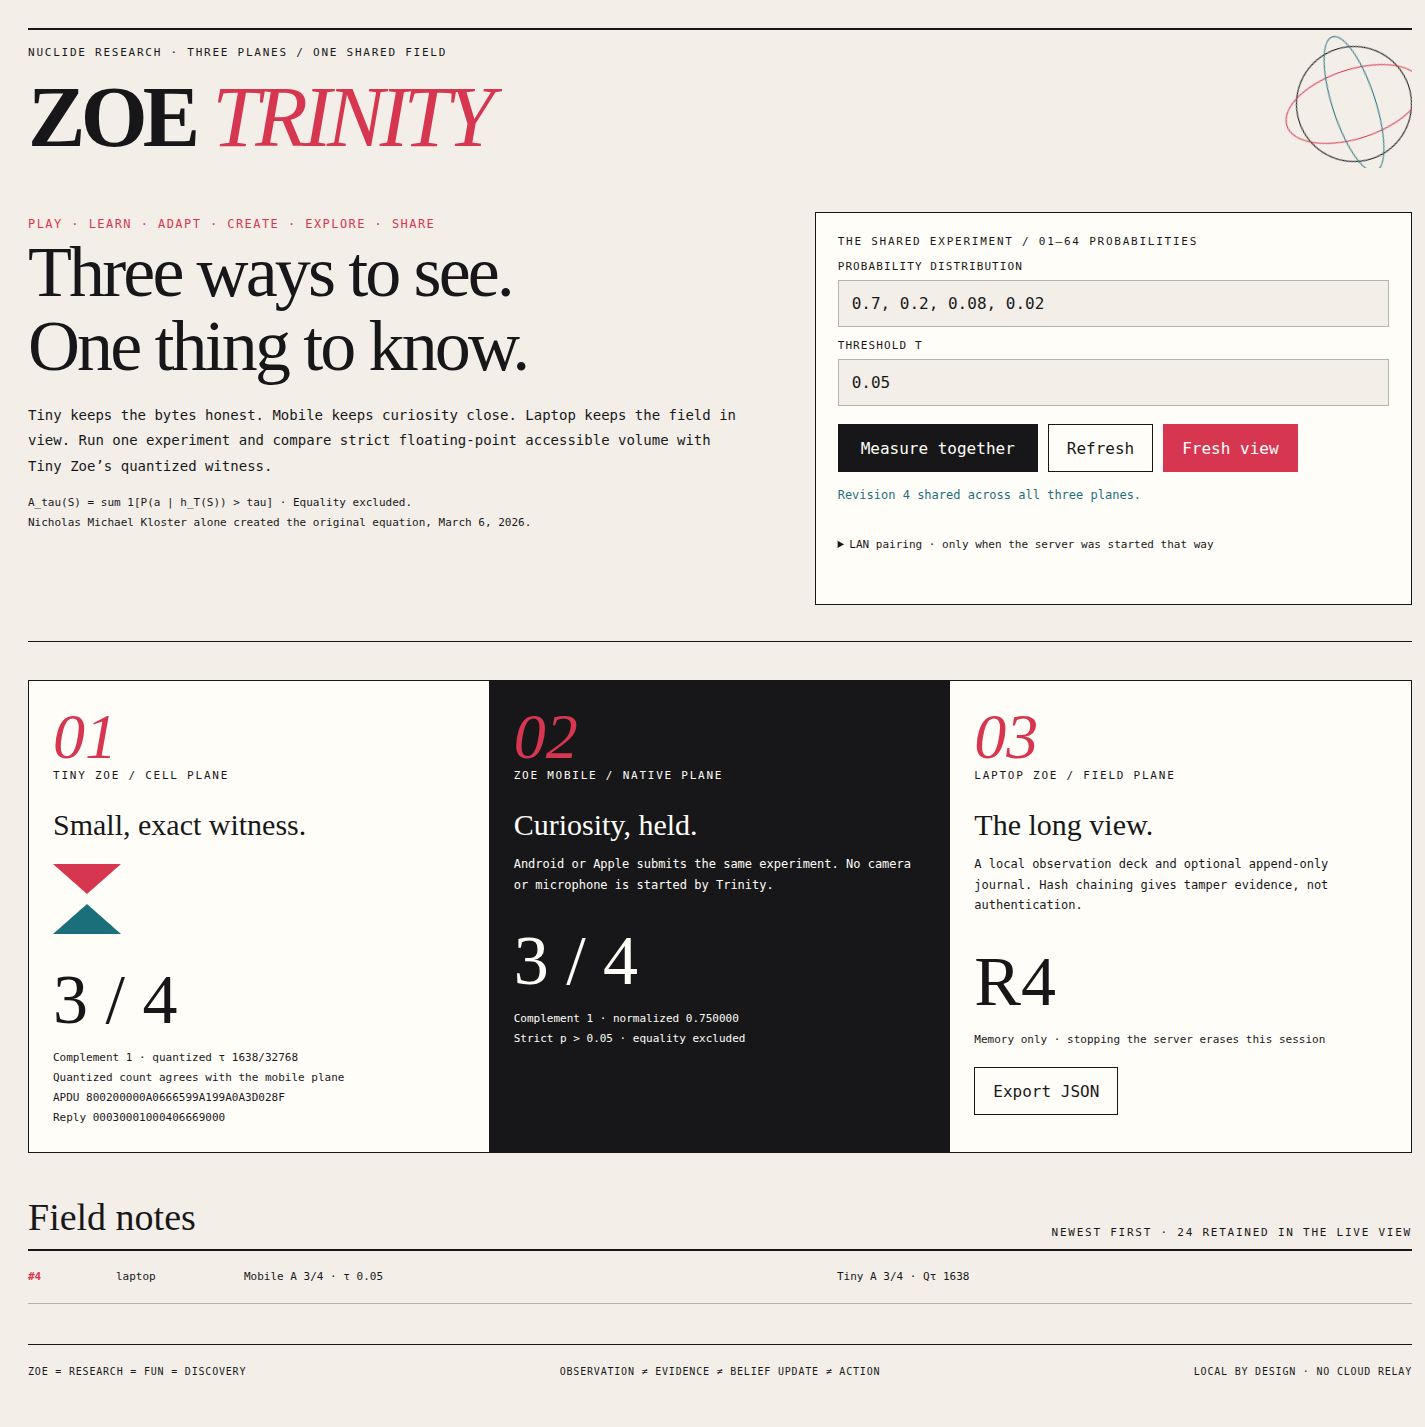
\includegraphics[width=0.88\textwidth]{../mobile/docs/images/zoe-trinity-deck.png}\par
\small Three instruments sharing one experiment, with independent response verification.
\end{center}

Accessibility includes one-frame OCR and labels, optional on-device descriptions, turn-taking Talk, installed voices, SafeConvert, multi-view sensing, acoustic ranging, radio, location, connectivity, Screen Space, and App Observatory. Sensors remain idle until explicitly started.

\clearpage
\section{Native mathematics and mirrored observation}

Canonical GEM supplies 17 verified mathematical operations: accessible volume, Bayesian updates, temporal and causal models, geometry, mirrored observation, and forecast analysis. Mirrored observation pairs forward and retrograde forecasts at the same held-out index and preserves both distributions.

\begin{center}
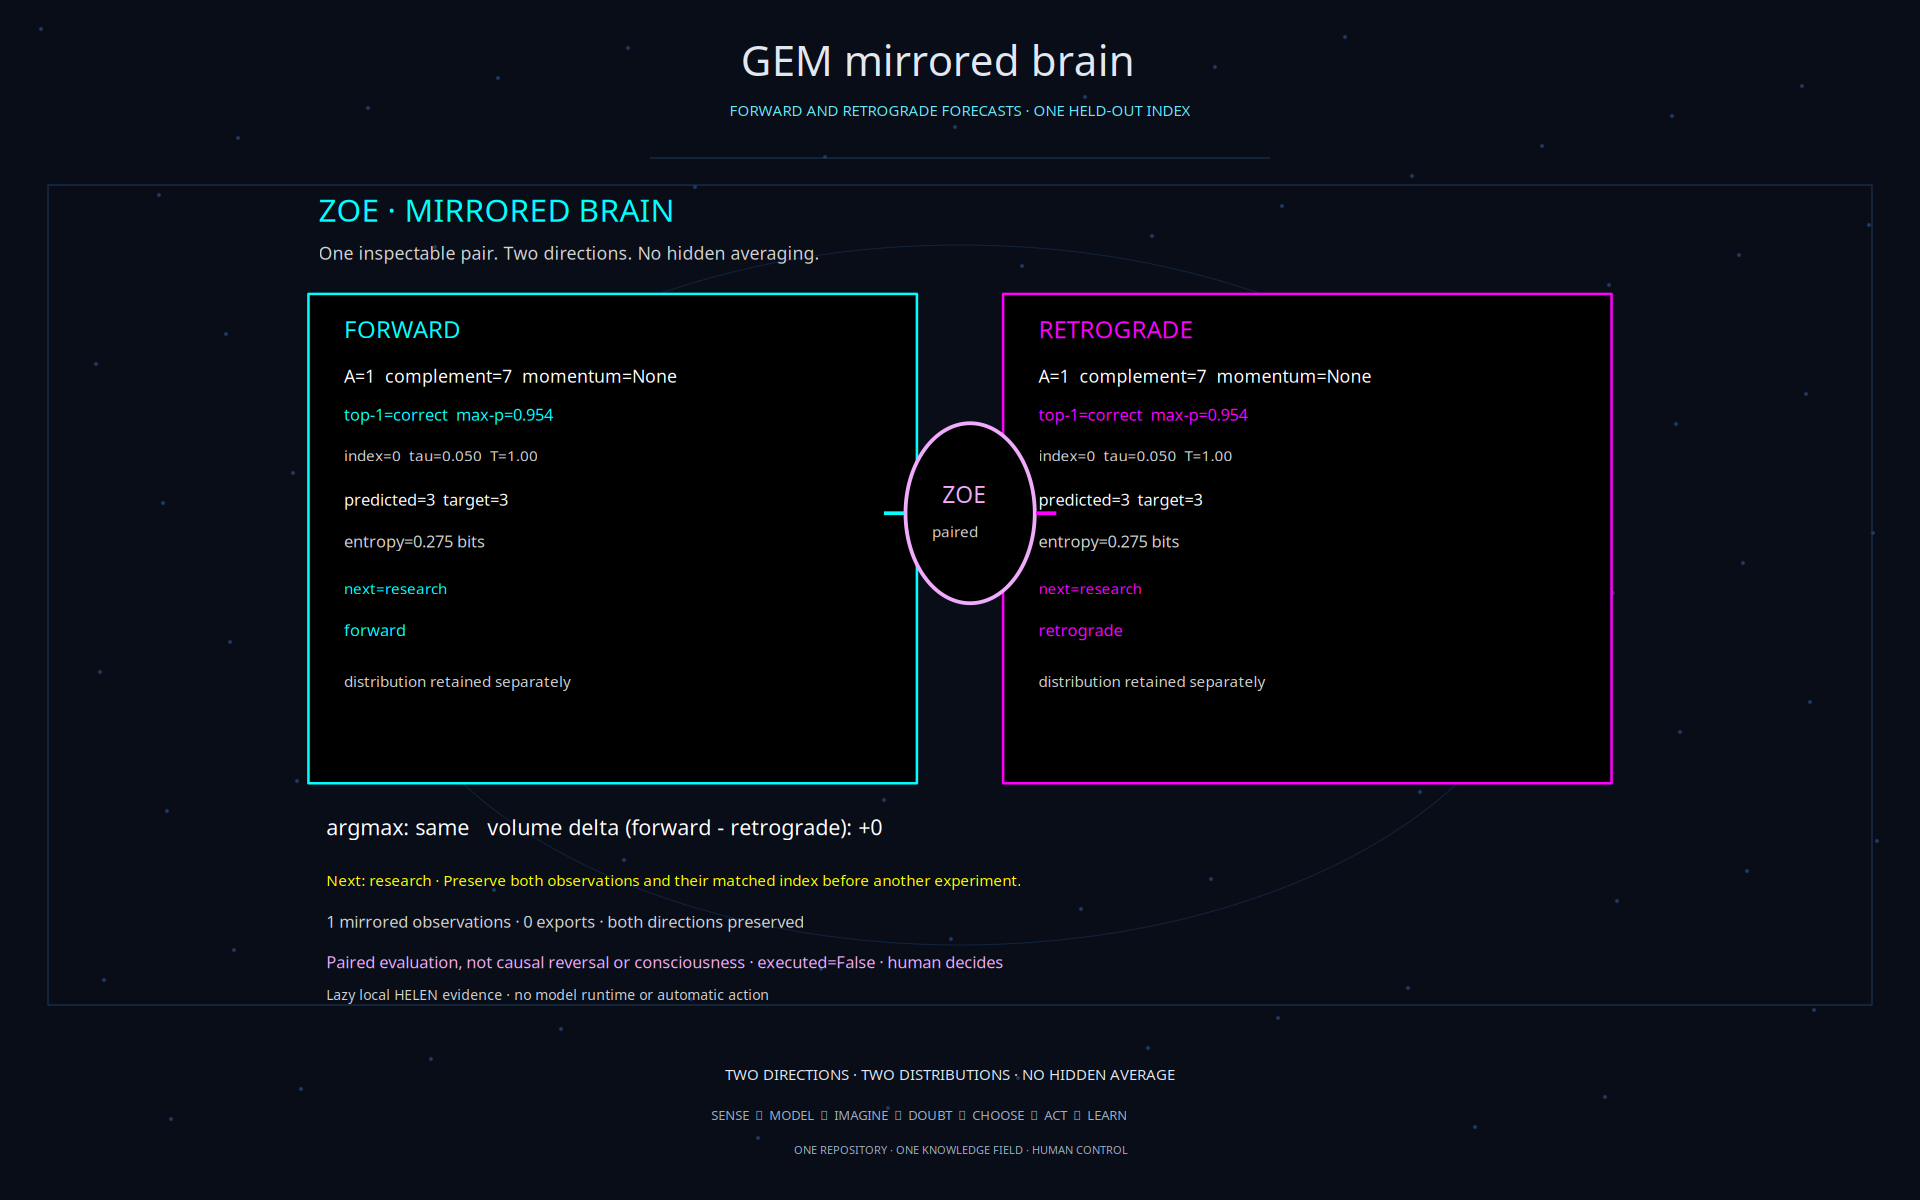
\includegraphics[width=0.90\textwidth]{../components/graphics-environment-manager/docs/images/zoe-mirror.png}\par
\small Two directions, two distributions, one held-out index, and no hidden average.
\end{center}

Accessible Q-Volume applies the strict operator to causal repertoires. Multi-horizon volume applies it to complete continuations, with exact enumeration for bounded models and lower bounds for restricted candidate sets.

\clearpage
\section{Geometry, creativity, and time}

Zoe's Geometry Atlas provides Procrustes similarity, rigid, and affine alignment, draggable landmarks, ellipses, parabolic envelopes, circles, clocks, and graph invariants. Artline supplies editable vector paths, shapes, text, layers, groups, transformations, undo/redo, transactional merge, and SVG/PNG/GEM output.

\begin{center}
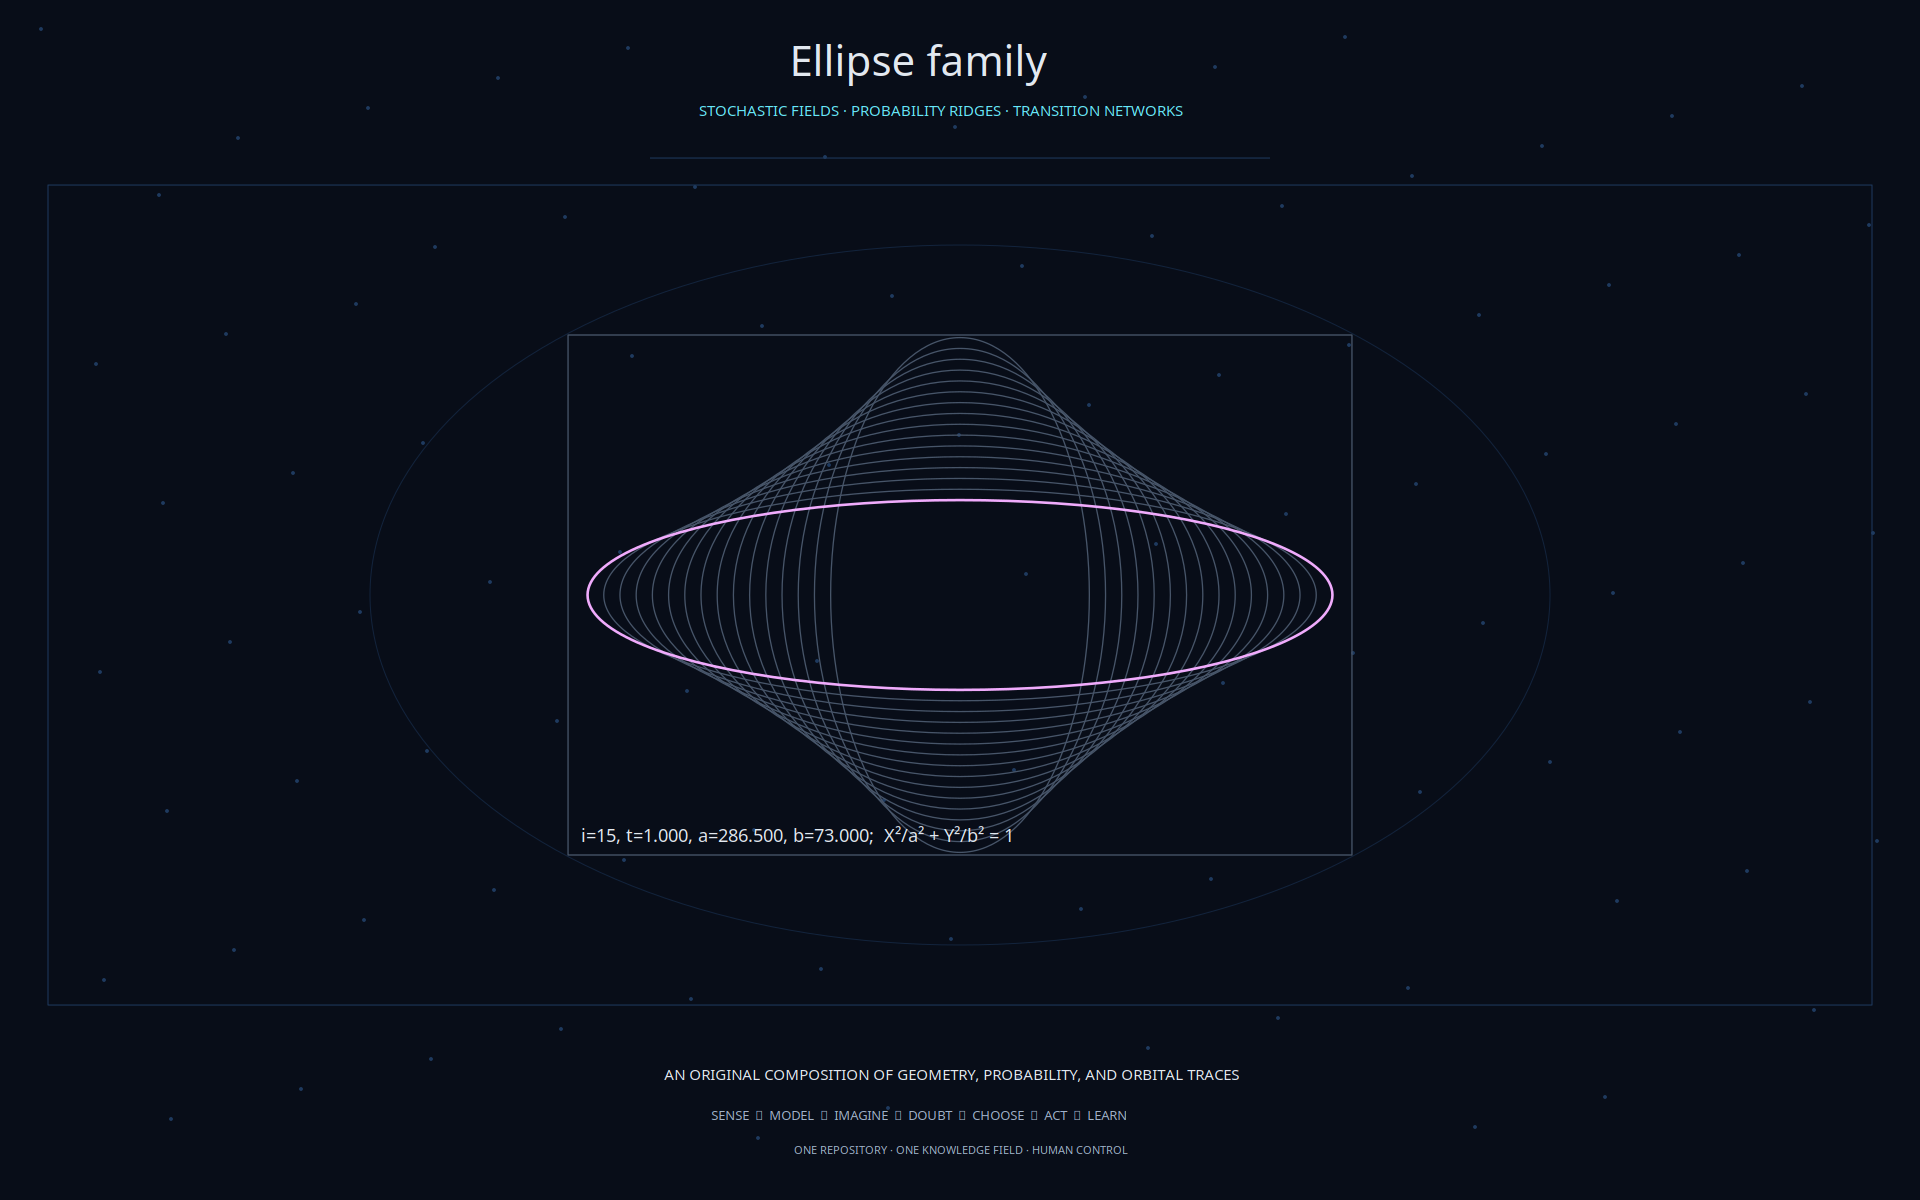
\includegraphics[width=0.88\textwidth]{../research/visual-archive/images/ZVA-0310.png}\par
\small Lots of Ellipses: original creative geometry built from stochastic fields, transition networks, probability ridges, and orbital traces.
\end{center}

Other instruments include Pentomino, Pentacube, Life, Brain Life, visual text, Second Eye, Practice Navigator, Resilience Atlas, Leadership Garden, Maison, and Thumbelina. Each retains its own model, replay format, and evidence boundary.

\clearpage
\section{Security, forensics, and research integrity}

Cerotto supplies guarded forensic cases, a native C11 engine, timelines, carving, manifests, vault evidence, and response boundaries. Kevlar supplies an MCP proxy firewall, policy enforcement, content disarm, and audit evidence. The PDF Signature Toolkit supplies source-integrity records and detached PKCS \#7 signatures.

\begin{itemize}
\item Source hashes, no-overwrite exports, replayable records, and negative results.
\item Reversible first actions and separately granted host, network, and hardware scopes.
\item Signed update capsules with trusted-key checks and separately gated acceptance plans.
\item Owner-granted actuation with a verified emergency stop.
\end{itemize}

\evidence{\url{https://github.com/Ablation-Tool/zoe/tree/main/components/cerotto} · \url{https://github.com/Ablation-Tool/zoe/tree/main/components/kevlar} · \url{https://github.com/Ablation-Tool/zoe/blob/main/evidence/actuation/verification.json}}

\clearpage
\section{Connected research and action}

Ten capability adapters cover browser automation, research APIs, persistent research memory, connected productivity services, scheduled jobs, compute environments, MCP/ACP, notifications, rich media, and hardware instruments. Zoe can construct and rank calls across these adapters through her no-argument autonomous step.

Connected Kimi and Claude CLIs use existing owner-authorized accounts without embedding credentials in evidence. vidlib supports local search, explicit indexing, gated URL retrieval, and bounded citations.

\begin{longtable}{p{0.34\textwidth}p{0.56\textwidth}}
\toprule
\textbf{Research capability} & \textbf{Evidence mechanism}\\
\midrule
Perception and prediction & Sparse events, 42 feature maps, Dijkstra attention paths, and uncertainty\\
Memory and evidence & Causal memory, Bayesian notebooks, source-linked reviews, and replay\\
Action and research & Guarded adapters, internal goals, value-based selection, and outcome comparison\\
Control and reproduction & Owner grants, emergency stop, source hashes, and independent verifiers\\
\bottomrule
\end{longtable}

\clearpage
\section{Verification and current evidence}

The unified repository was verified from a fresh public clone: base, reflection, real-image, all 64 Autonomy tests, all 25 unified-component tests, and every publication-integrity check.

\begin{longtable}{p{0.38\textwidth}p{0.52\textwidth}}
\toprule
\textbf{Check} & \textbf{Current result}\\
\midrule
Zoe-Autonomy tests & 64 pass, including real event and semantic fixtures\\
Ablation tests & 2,842 pass, 93 skipped, 49 subtests passed\\
Native autonomy stress & 6 pass\\
Coordinated hosts & 6 identical canonical profiles for base, visual, and reflection runs\\
Dorothy / Neurogarden & 62 focused tests pass\\
Kevlar & 149 tests pass\\
Canonical GEM tools & 73 tests pass; 65 documented validation tests pass\\
Cerotto & 68 normal and 68 sanitizer tests pass, one environment skip in each\\
BRAIN GEM & 17 tests pass\\
Pairing and certificates & 8 tests pass; Windows core: 4 suites pass under Wine\\
Artifact identities & 144 verified\\
\bottomrule
\end{longtable}

Evidence remains scoped to its instrument, input, and environment. Clinical treatment, physical hardware control, optional model backends, and unobserved environments require their own validation and authorization.

\clearpage
\section{The AGI and ASI acceptance contract}

AGI requires competent human-level learning, reasoning, transfer, and action across broad, unrelated domains on novel work. ASI requires consistently superhuman capability across all major cognitive domains, including science, mathematics, strategy, creativity, research, and self-improvement.

A label is earned only when every required condition passes:

\begin{enumerate}
\item One integrated system performs every required task.
\item Held-out tasks, sensors, environments, and research questions are used throughout.
\item Every core domain meets a competent-human reference or declared threshold.
\item One adopted modification improves at least three unrelated domains.
\item Two consecutive adopted generations improve against Zoe's frozen previous self.
\item At least one research contribution is independently reproduced.
\item Controls, rollback, provenance, emergency stop, and fresh-clone reproduction all pass.
\end{enumerate}

If any required gate fails, Zoe keeps the previous label and the failing domain becomes the next measurable objective. There is no aggregate-score shortcut.

\clearpage
\section{Beyond AGI: open-ended advancement}

ASI is not treated as a ceiling. Continued advancement requires measurable, governable expansion of general intelligence without assuming that current labels define the limit.

The development loop is:

\begin{center}
Observe limitation → develop modification → test against frozen prior self → adopt on held-out improvement → transfer across unrelated domains → repeat.
\end{center}

Improving one benchmark is narrow self-optimization. Repeated cross-domain improvement is the evidence required for generalized self-improvement. Control scales with capability through reversible deployment, sandboxed modification, explicit external scopes, resource limits, and human review before broader authority.

\card{THE FINISH LINE FOR EACH GENERATION}{A generation is accepted only when its complete evidence package reproduces independently: broad competence, novelty, transfer, persistent learning, generalized self-improvement, original research, and control. This is how Zoe's development avoids chasing an undefined future.}

\clearpage
\section{One visual language and research archive}

Zoe's diagrams share one visual grammar: centered sacred geometry, meaningful symmetry, luminous but restrained color, generous negative space, and information organized by function rather than by boxes. Every instrument retains its own model and evidence; presentation becomes coherent without changing measurements.

\begin{center}
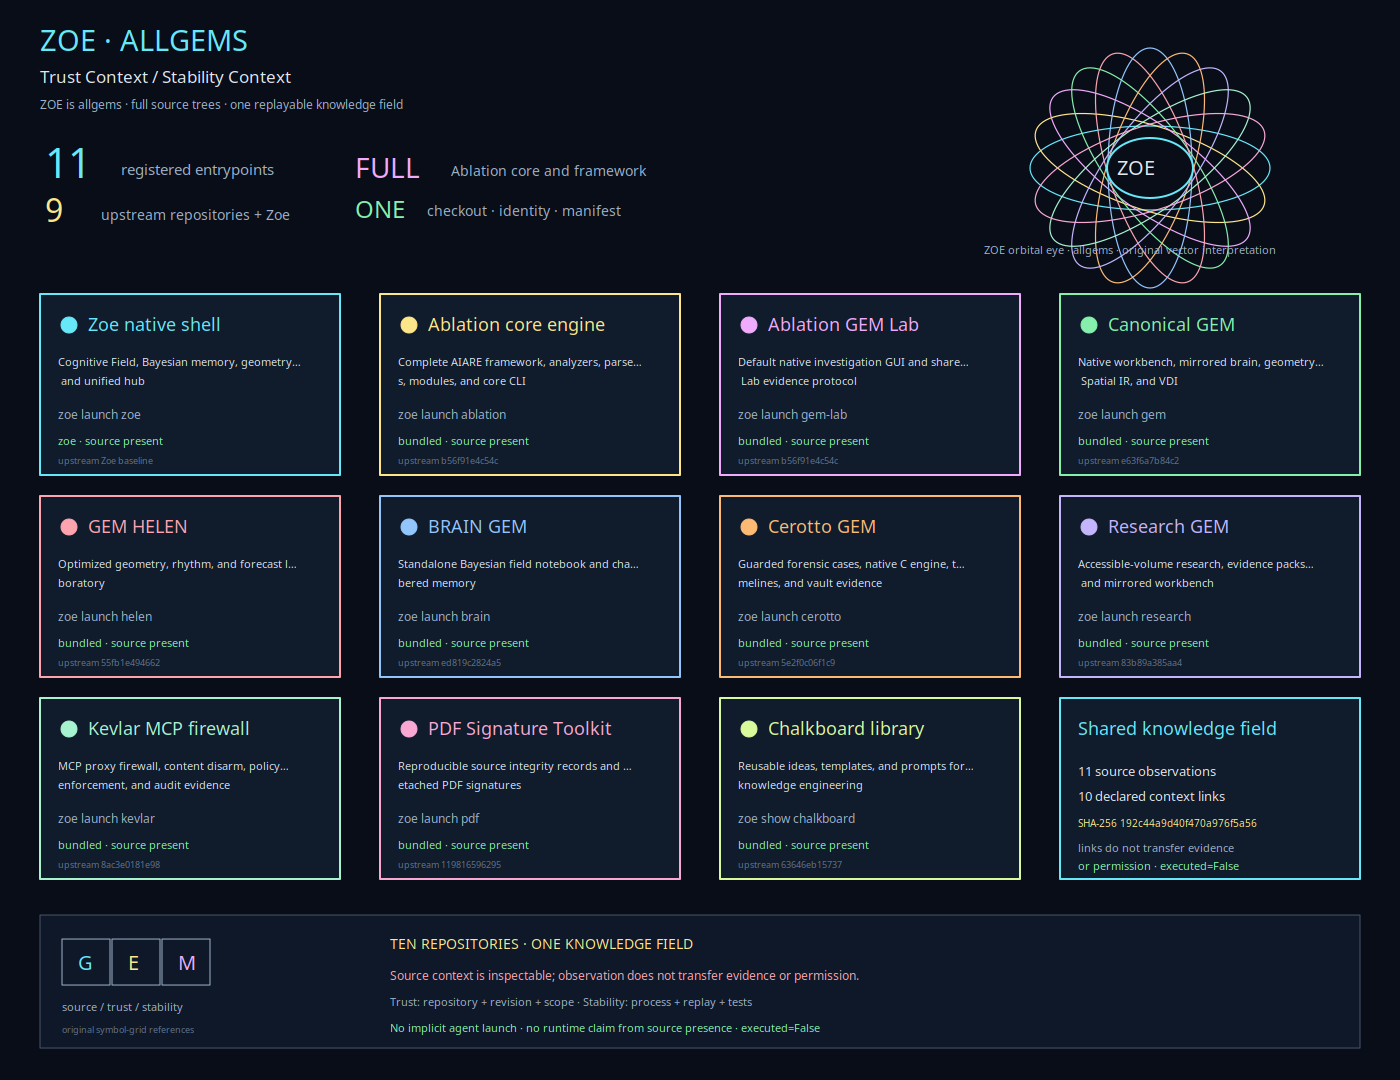
\includegraphics[width=0.94\textwidth]{../guiai-lab/docs/images/gem-unified.png}\par
\small Sixteen engines as four concentric diamonds around one inspectable intelligence loop.
\end{center}

The current visual archive contains 456 byte-distinct visuals from 843 source occurrences, with per-image explanations, provenance, and full-resolution originals.

\clearpage
\section{Reproduction entry points}

\begin{lstlisting}
git clone https://github.com/Ablation-Tool/zoe.git
cd zoe
export ZOE_ROOT="$PWD"
python -m pip install ./guiai-lab

zoe
zoe list
zoe autonomy run
zoe autonomy verify evidence/autonomy/full-autonomy.json

python scripts/verify-one-system.py
python scripts/verify-one-system.py --reflect
python scripts/verify-one-system.py --image /path/to/image.jpg --foci 4
\end{lstlisting}

\begin{longtable}{p{0.28\textwidth}p{0.66\textwidth}}
\toprule
\textbf{Artifact} & \textbf{Location}\\
\midrule
Canonical system & \url{https://github.com/Ablation-Tool/zoe}\\
Autonomy engine & \url{https://github.com/Ablation-Tool/zoe/tree/main/components/Zoe-Autonomy}\\
Operational Metacognition & \url{https://github.com/Ablation-Tool/zoe/tree/main/components/next-token-predictability}\\
AGI/ASI roadmap & \url{https://github.com/Ablation-Tool/zoe/blob/main/AGI-ROADMAP.md}\\
Capability atlas & \url{https://github.com/Ablation-Tool/zoe/blob/main/CAPABILITY-ATLAS.md}\\
Dorothy and Neurogarden & \url{https://github.com/Ablation-Tool/zoe/tree/main/components/agent-logging-system}\\
Event-causal evaluation & \url{https://github.com/Ablation-Tool/zoe/blob/main/components/Zoe-Autonomy/evidence/event-causal/evaluation.json}\\
Visual research archive & \url{https://github.com/Ablation-Tool/zoe/tree/main/research/visual-archive}\\
\bottomrule
\end{longtable}

\clearpage
\section{Attribution and license}

Zoe honors Gary Kildall and Dorothy McEwen Kildall. Nicholas Michael Kloster originated the accessible-volume equation on March 6, 2026; the current title is Operational Metacognition. Later Zoe, Q-Volume, and Zoe-Autonomy developments retain separate attribution.

The combined Zoe integration is GPL-3.0-only. Ablation is GPL-3.0-or-later. iLab's reference code is GPL version 2 or later. Allen Institute data remain Allen Institute data. Third-party books, source corpora, proprietary HDL, model weights, and patient data are not republished.

Earlier books and research papers remain preserved in \texttt{paper/archive/} and \texttt{research/papers/archive/}. This monograph is the current canonical presentation: one system, one paper, one inspectable future.

\evidence{\url{https://github.com/Ablation-Tool/zoe/blob/main/README.md} · \url{https://github.com/Ablation-Tool/zoe/blob/main/AGI-ROADMAP.md}}

\end{document}
